《当代央地关系》之土地金融与土地整理。

本节几乎照摘周飞舟和谭飞智所著《当代中国的中央地方关系》。笔者对原文个别不同
看法,用脚注加以说明。

自改革开放以来,我国工业化、城镇化推进速度越来越快,大量耕地农用地被占用是土
地财政\footnote{“土地财政”四字为笔者所加。}发展的必然要求。尤其是进入21世纪以来,
各地土地财政带来大拆大建,形成规模不小的失地农民群体,频发的群体性事件成为危
害社会稳定的重要因素。自中央层面来看,基于保障\textbf{国家粮食战略安全}\footnote{原文是
“国家粮食安全”,笔者加入“战略”二字,突出粮食安全地位。}以及维持改革以来
确立的家庭联产承包责任制的基本经营组织方式的要求,实行严格的耕地保护制度,以
占补平衡为代表的系列政策应运而生,\textbf{18亿亩耕地红线}作为一项政治任务贯穿而下,
实行一把手问责制。

\subsection{耕地占补平衡}

1997年4月,中共中央国务院发布11号文《关于进一步加强土地管理、切实保护耕地的通
知》,明确提出省(区市)必须保持耕地总量动态平衡的要求,同时确定了实行占用
耕地与开发复垦\footnote{土地复垦是指对生产建设活动和自然灾害损毁的土地,采取整治措施,
  使其达到可供利用状态的活动。}挂钩的政策,首次明确提出“耕地占补平衡”的概念。

随后在1998年8月,《中华人民共和国土地管理法》再次修订,明确提出“实行占用耕地
补偿制度”,要求占用耕地与开发复垦耕地相平衡。

1999年2月4日,《关于切实做好耕地占补平衡工作的通知》(国土资发〔1999〕39号)要
求确保建设占地“\textbf{占一补一}”,逐步实现耕地占用的\textbf{先补后占、占优补优、不补不
  占}。自此,耕地占补平衡政策开始在全国各地大规模实施。

2006年以前,占补平衡考核采取的是“\textbf{算大帐}”的方法——以区域为单位,考核区域内
的总占总补平衡。这种方法存在的漏洞是,很多建设用地项目并没有实现法律所规定的
占补平衡,建设用地占用耕地项目单位的补充耕地与土地开发整理脱钩。同时,由于区
域内的占补平衡考核仅仅关注于数量,一些建设项目\textbf{占优补劣}的现象比较突出。

2006年6月8日,国土资源部第3次部务会议通过了《耕地占补平衡考核办法》,于当
年8月1日起施行。“耕地占补平衡考核,\textbf{以建设用地项目为单位进行}”“耕地占补平
衡,实行占用耕地的\textbf{建设用地项目与补充耕地的土地开发整理项目挂钩}制度。”不再
采取大锅饭式的算大账。这一管理思路,为后来的增减挂钩所延续,即采用“\textbf{封闭运
  行}”的项目制运作模式,

随着工业化、城镇化的大势所趋,\textbf{“保耕地红线”成为地方政府沉重的政治负担和资金负
担。}耕地占补平衡政策自出台以来,在各地具体实施过程中主要存在:耕地的“\textbf{实占虚
补}”;补充耕地的“\textbf{实优虚劣}”以及\textbf{农地非农化和非粮化}的风险。耕地占补平衡制度实
行以来,各地实际工作中建设占用耕地长期以“先占后补”和“边占边补”方式为主,
加上对补充耕地的监督力度不够,导致建设占用耕地占而不补、占多补少的问题经常发
生。国土资源部因此颁布《关于进一步加强土地整理复垦开发工作的通知》,规定
从2009年开始,除国家重大工程可以暂缓外,非农占用耕地全面实行“\textbf{先补后占}”。

% 从地方政府角度出发,其更多的是从如何提高土地生产效益的角度出发的,因此如果单
% 纯地维持原有以粮食为主的种植结构难以达到提高效益的目的,转变生产结构成为必然
% 的选择,农地非农化、非粮化在所难免。所谓粮食安全的担忧也并非地方所考虑的问题。
% 在这一点上,中央与地方之间的矛盾凸显。

由于耕地的开垦整理需要一定的工程周期,因而由“先占后补”到“先补后占”的转变,
开启了\textbf{耕地占补平衡指标化}的进程,各地纷纷建立\textbf{占补平衡指标储备库}。提前储
备补充耕地,需新增建设用地时再从库中支取“指标”。

% 中国耕地红线粮食战略安全和土地金融的交织摩擦,使地区\textbf{狂热开发}建设用地的意
% 图受限\footnote{此句为笔者所加。以中国为一整体的角度来考虑,各地重复建设、大干快上,
% 工业用地扭曲的拿地或租赁价格、房地产的癫狂实属狂热无疑。},尤其是经济发达地
% 区与产粮大省更加受限于补充耕地资源较少。

% 从另一各方面来说,耕地红线也使可转化为新增建设用地的农地更加稀缺,加重了土地
% 金融的严重程度。\footnote{此句为笔者所加。}

\subsection{土地置换与指标折抵}

中央、省、市、县、乡五级政府的五级规划与年度建设占用耕地计划指标等限制了各级
地方政府对于新增建设用地、发展土地金融的强烈渴求,与中央严格土地制度框架出现
较尖锐矛盾,违法占地屡禁不止,中央政府为此开了以农用土地整理换取新增建设用地
的“口子”。

1999年10月,《国土资源部关于土地开发整理工作有关问题的通知》(国土资发
〔1999〕358号)提出土地置换和指标折抵。

\begin{description}
\item[土地置换] 促进农村居民点向中心村和集镇集中、乡镇企业向工业小区集中,选定新
  址\textbf{建设需要占用其他耕地}时,可以与腾出来的\textbf{旧址整理后增加的耕地}进行置换,实行
  这种方式置换的其建设用地\textbf{不占用年度建设占用耕地计划指标}。


\item[百分之六十指标折抵] 实现耕地占补平衡的地区,可以用通过土地整理\textbf{新增耕地面积
  的百分之六十指标},向上级土地行政主管部门申请一定数量的\textbf{预留建设占用耕地指标},
  用于本地区必需的非农建设。但必须按规划用地,并要严格检查,适当控制。
\end{description}

这两项政策“指标的使用并\textbf{不占用当年的年度建设用地指标},因而受到各地方政府的
欢迎……也是城乡建设用地增减挂钩政策出台的前奏”。

但地方政府仍感受到五级区域对于发展建设用地限制较大:发达地区可供补充耕地量匮
乏,不能满足新增建设用地需求;一般为10--15年的土地规划无法更好预见未来发展,
不可占用基本农田\footnote{基本农田:为了切实保护耕地,国家把按照一定时期人口和社会经
  济发展对农产品的需求,以及对建设用地的预测而确定的\textbf{长期或一定时期内不得占
    用的耕地}称为基本农田。}使大块建设用地项目难以落地。于是一些省开始省内跨
区域操作,实现了较为系统性变通的是浙江省,一些人称之为“\textbf{浙江模式}”。简而言
之就是浙江省将一些指标统筹在省或市以内,不下沉分解至各县各乡;并且各市之间可
以交易指标,落后地区大量土地整理用以补充耕地,发达地区向落后地区购买耕地指标
专心发展建设用地。详细了解可见汪晖、陶然《论土地发展权转移与交易的 “浙江模
式”——制度起源, 操作模式及其重要含义》。


\begin{quotation}
  对浙江在土地发展权转移和交易上的改革探索,不仅学界有论述质疑浙江的做法
  是\textbf{规避中央政府基本农田审批权和新增建设用地土地有偿使用费,导致基本农田质
    量下降和建设用地总量失控}(谭峻等,2004 年),中央政府也存在不少担心。

  欠发达地区为了折抵指标过度投资土地整理,甚至在新增耕地比例上弄虚作假,或发
  达地区通过购买折抵指标无限制扩张城市和工业园区用地。

  浙江省基本农田集中置换和易地代保政策\footnote{即基本农田易地代保:简而言之,发达市
    县有偿购买落后市县的基本农田,以便消除本市县相应面积、质量的基本农田保护,
    新增大块连续建设用地。}在国土资源部《关于进一步采取措施落实严格保护耕地制度的通
  知》(国土资发〔2003〕388 号和国务院办公厅《关于深入开展土地市场治理整顿严格
  土地管理的紧急通知》(国办发明电〔2004〕20 号)公布后停止执行;折抵指标政策也
  在《国务院办公厅关于严格执行有关农村集体建设用地法律和政策的通知》(国办发
  〔2007〕71 号)颁布后停止执行。\cite{wangzhejiang}
\end{quotation}




\todo[inline]{浙江模式其实就是市县级土地金融的扩大版,大国大城其实就是浙江模
  式的扩大版?参考LaTeX源文件中以下被注销部分。自由派认为行政主导要继续让位
  给市场自由流动。}

\subsection{城乡建设用地增减挂钩}

\begin{quotation}
  按照2004年10月21日国务院下发的《关于深化改革严格土地管理的决定》,即“鼓励
  农村建设用地整理,\textbf{城镇建设用地}增加要与\textbf{农村建设用地}减少相挂钩”。

  (4年陆续增加试点后,)2008年6月27日,国土资源部印发《城乡建设用地增减挂钩
  试点管理办法》,明确提出了“城乡建设用地增减挂钩是指依据土地利用总体规
  划,\textbf{将若干拟整理复垦为耕地的农村建设用地地块(即拆旧地块)和拟用于城镇建
    设的地块(即建新地块)等面积共同组成建新拆旧项目区}(以下简称项目区),通
  过建新拆旧和土地整理复垦等措施,在保证项目区内各类土地面积平衡的基础上,最
  终实现增加耕地有效面积,提高耕地质量,节约集约利用建设用地,城乡用地布局更
  合理的目标。”其实仔细比较增减挂钩政策与之前我们所分析的建设用地指标置换政
  策其在表述上和本质上相类似,而这也反映了中国改革中政策制定的延续性和探索性。

  同时138号文批复下达了第二批试点项目(共10246公顷,合15.368万亩),项目区以
  项目区备选方式下达。2009年3月5日,《国土资源部关于2009年第一批城乡建设用地
  增减相挂钩周转指标的批复》(国土资函[2009]299号),对河北、内蒙古、辽宁、吉
  林、黑龙江、福建、江西、河南、湖南、广东、广西、云南、宁夏13省(区),批复
  下达周转指标15.275万亩(合10183.3公顷)。2013年10月23日下午,国土资源部部长、
  党组书记、国家土地总督察姜大明主持召开第15次部长办公会,审议并原则通
  过2013年城乡建设用地增减挂钩指标分解下达方案,共批准29个省份开展增减挂钩试
  点,全国共安排城乡建设用地增减挂钩指标90万亩。\cite{yangdi}

  指标计算公式:增减挂钩周转指标=拆旧区总面积-农民集中居住小区占地面积=项目区
  中建新地块可占地面积(见\cref{fig:zengjianguagou})。所谓“\textbf{周转指标}”其
  在实质上是一种指标“\textbf{预借}”或“\textbf{透支}”制度。拆旧复垦是一项非常庞大的工
  程,短期内难以完成,因此不需要拆旧区完成耕地复垦工作之后,建新区才能够进行
  城镇开发建设。也正是在这个意义上才有了指标“\textbf{周转}”的概念,一般要求,指标
  三年归还。
\end{quotation}

\begin{figure}[ht]
  \centering
  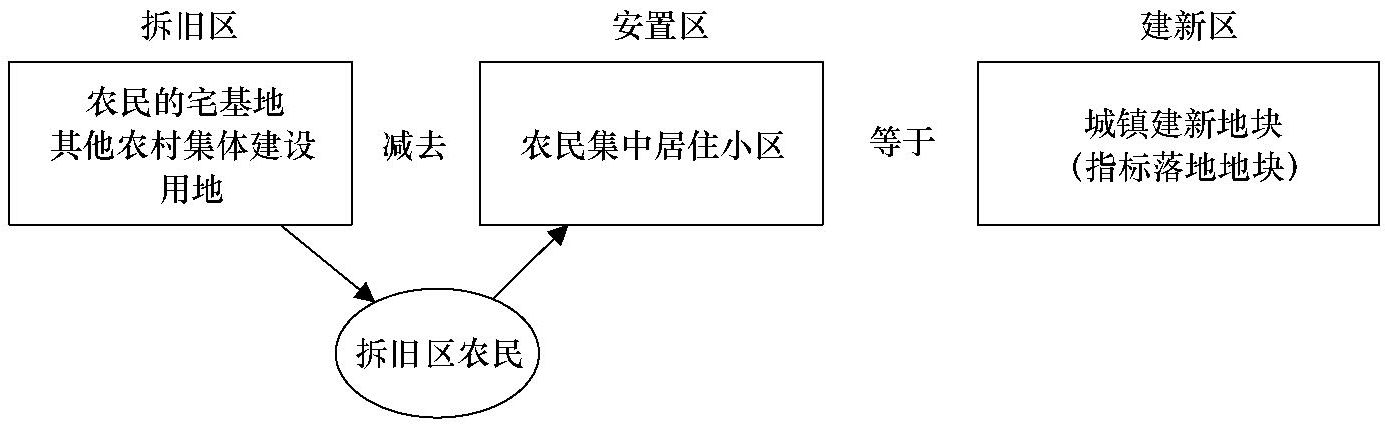
\includegraphics[width=0.9\linewidth]{figures/zengjianguagou.jpg}
  \caption{\label{fig:zengjianguagou}城乡建设用地增减挂钩政策示意图}
  \capsource{周飞舟、谭飞智\quad 《当代中国的中央地方关系》}
\end{figure}


%
% 在全国范围内推广“土地发展权转移和交易”的浙江模式,不仅能增加发达地区的土地
% 利用和欠发达地区收入,也能通过市场化的自愿指标交易,节省(政府或管制者)进行
% 耕保的信息和监督成本。从发达地区角度看,不仅可以通过市场化方式大大缓解这些地
% 区的用地指标紧张局面,也可促进起通过城市化来吸纳更多的农村与欠发达地区人口进
% 入城市就业和定居,降低欠发达地区人口对当地耕地压力和欠发达地区发展本地非农产
% 业、占用耕地的压力。从那些具有更多耕地资源禀赋的欠发达地区角度看,他们可以通
% 过土地发展权交易获得宝贵的耕地保护乃至农业发展资金,这不仅促进了区域之间财力
% 的转移和区际财力平等,也有助于欠发达地区农业比较优势的充分发挥。而限于浙江这
% 个发达省份内部的跨地市土地发展权交易,必然会因为\textbf{浙江本省耕地资源的有限性}而
% 使得交易操作空间较小。到一定阶段后,省内的发达地市或者买不到指标,或者购买成
% 本过高,结果是还不如在建设用地上进行\textbf{违规操作}。实际上,从近年的发展来看,浙
% 江省内进一步进行“折抵指标交易”,“耕地易地有偿代保”和“异地耕地占补平
% 衡”的空间已经日渐缩小,市场开始趋向\textbf{萎缩}。因此,如果上述土地发展权转移和交
% 易的改革措施不能够在全国范围内推广,建设用地计划管理体制改革的“浙江模式”即
% 使在本省内也将无法持续下去。因此,浙江模式的全国含义,就是它的完善和推广,将
% 不仅有助于全国耕地资源保护目标的实现,有助于我国正在进行的主体功能区规划目标
% 的实现,而且也将有助于提高我国土地利用、人口、劳动力跨区配置的效率,从而同时
% 提升我国整体经济发展的效率和平等。

% 实际上,由于多种原因,浙江既有的土地利用政策改革已经部分被叫停,比如基本农田集中置换和易地代
% 保政策在国土资源部《关于进一步采取措施落实严格保护耕地制度的通知》(国土资发[2003]388 号)和国
% 务院办公厅《关于深入开展土地市场治理整顿严格土地管理的紧急通知》(国办发明电[2004]20 号)公布后
% 停止执行;折抵指标政策也在《国务院办公厅关于严格执行有关农村集体建设用地法律和政策的通知》(国
% 办发〔2007〕71 号)颁布后停止执行。

韩长赋: 中国农村土地制度改革

耕地退化、污染严重,一些地方占好地、补坏地,占水地、补旱地,2016 年全国优高
等耕地面积仅占 29. 5%。


http://cn.chinagate.cn/news/2020-06/05/content_76131126.htm

https://www.gov.cn/zhengce/2018-08/13/content_5313406.htm
国务院办公厅印发《跨省域补充耕地国家统筹管理办法》和《城乡建设用地增减挂钩节
余指标跨省域调剂管理办法》。进一步明确了跨省域补充耕地资金要全部用于巩固脱贫
攻坚成果和支持实施乡村振兴战略,从而充分发挥经济发达地区和资源丰富地区资金、
资源互补优势,推动区域协调发展。
